

\documentclass[12pt,a4paper]{report}
\usepackage{graphicx}
\usepackage[utf8]{inputenc}
\usepackage[T1]{fontenc}
\usepackage[a4paper,top=3cm,bottom=2cm,left=3cm,right=3cm,marginparwidth=1.75cm]{geometry}
\usepackage[spanish]{babel}
\selectlanguage{spanish}
\usepackage{fancyhdr}

% quitar el 0.
\renewcommand\thesection{\arabic{section}}

% aqui definimos el encabezado de las paginas pares e impares.
\lhead[x1]{
\includegraphics[width=1cm]{./images/epis}}
\chead[y1]{}
\rhead[z1]{Inteligencia de Negocios}
\renewcommand{\headrulewidth}{1pt}

% aqui definimos el pie de pagina de las paginas pares e impares.
\lfoot[a1]{Ing. Patric Cuadros}
\cfoot[c1]{}
\rfoot[e1]{\thepage}
\renewcommand{\footrulewidth}{1pt}

\pagestyle{fancy} 



\begin{document}
\begin{titlepage}
	\centering
	
\includegraphics[width=4cm]{./images/upt}\par\vspace{1cm}
	{\scshape\LARGE\huge\bfseries Universidad Privada de Tacna \par}
	{\scshape\LARGE Escuela de Ingenieria de Sistemas \par}
	\vspace{1cm}
	{\scshape\Large Inteligencia de Negocios\par}
	\vspace{0.5cm}
	{\huge\bfseries Aprendizaje Supervisado \par}
	\vspace{1cm}

	{\Large\itshape PRESENTADO POR:\par}
	{\Large\itshape Lopez Mamani, Aldo Franco \par}
	{\Large\itshape Condori Quisoi, Jesus Humberto\par}
	{\Large\itshape Vilca Chambilla, Wilfredo\par}
	{\Large\itshape Cayetano Chiri, Evelyn Paola\par}
	{\Large\itshape Zavala Venegas, Kuis Angel\par}
	{\Large\itshape Vilca Mamani, Elisban\par}




	\vfill
	Docente\par
	Ing. Patrick Cuadros\textsc{Brown}

	\vfill

% Bottom of the page
	{\large \today\par}

\end{titlepage}
%% Aquí podemos añadir un resumen del trabajo (o del artículo en su caso) 

\begin{abstract}
\centering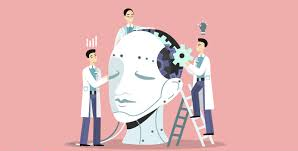
\includegraphics[width=16cm]{./images/10}\par\vspace{12cm}
\end{abstract}



\begin{abstract}
La inteligencia, en pleno siglo XXI, trasciende las fronteras de la mente. Mucho escuchamos decir que ahora los computadores son más inteligentes que los cerebros y que pronto los robots sustituirán a los humanos para pasar a dominar el mundo.
Está muy arraigada la creencia de que por más inteligente que pueda ser un computador, nunca podrá tener la capacidad de pensar. Sin ánimos de fatalismo, el aprendizaje automático ha revolucionado de forma decisiva el campo de la computación, facilitando la realización de todo tipo de tareas de forma digital y no manual. El aprendizaje automático, también conocido en inglés como machine learning, es un campo de la computación que lleva a otro nivel a la inteligencia artificial: hace que las computadoras aprendan a pensar.
No, no es tan literal. Los computadores no desarrollaron un cerebro y ahora tienen emociones. Simplemente el machine learning desarrolla algoritmos que hacen que las máquinas puedan aprender por su cuenta y responder a determinadas preguntas con bastante certeza. Para desarrollar estos algoritmos, existen dos modalidades: aprendizaje supervisado y no supervisado.

\end{abstract}

\begin{abstract}
\centering Abstract

La selección de una función de distancia adecuada es fundamental para los algoritmos de aprendizaje basados en instancias. Dicha función de distancia influye en el éxito o el fracaso de estos algoritmos. Recientemente se ha demostrado que incluso una transformación lineal simple de los atributos de entrada puede llevar a mejoras significativas en los algoritmos de clasificación como k-Noc. Más cercano (k-NN). Una de las aplicaciones principales de estos algoritmos es la hibridación con aplicaciones basadas en instancias. aprendiendo algoritmos y, en ese sentido, aprendiendo una métrica de distancia para la aplicación en cuestión y no utilizando una función de distancia general; que ha demostrado mejorar los resultados de aprendizaje. 

\end{abstract}
%% Iniciamos "secciones" que servirán como subtítulos
%% Nota que hay otra manera de añadir acentos


\addcontentsline{toc}{chapter}{Índice general}
\tableofcontents
\newpage

\section{Introducción}
El aprendizaje supervisado puede generar modelos de dos tipos. Por lo general, genera una función que transforma los datos de entrada en los resultados deseados.
Con el fin de resolver un determinado problema de aprendizaje supervisado (por ejemplo, aprender a reconocer la escritura) uno tiene que considerar varios pasos:
\begin{itemize}
\item Determinar el tipo de ejemplos de entrenamiento. Antes de hacer cualquier otra cosa, hay que decidir qué tipo de datos se va a utilizar para entrenar el modelo. Por ejemplo, podría ser un único carácter a mano, una palabra completa escrita a mano, o toda una línea de escritura a mano.
\item Reunir un conjunto de entrenamiento. El conjunto de necesidades de formación a las características propias del uso del mundo real de la función. Por lo tanto, un conjunto de objetos de entrada que se recopila y salidas correspondientes se recogen también, ya sea humana o de los expertos a partir de mediciones.
\item Determinar la función de ingreso de la representación de la función aprendido. La precisión de la función aprendida depende en gran medida de cómo el objeto de entrada está representado. Normalmente, el objeto de entrada se transforma en un vector de características, que contiene una serie de características que son descriptivos del objeto. El número de características no debe ser demasiado grande, a causa de la maldición de la dimensión, pero debe ser lo suficientemente grande como para predecir con precisión la salida.
\item Determinar la estructura de la función adecuada para resolver y el problema y la técnica de aprendizaje correspondiente. Por ejemplo, se podría optar por utilizar red neuronal artificial o un árbol de decisión.
\item Completar el diseño. El ingeniero a continuación, ejecuta el algoritmo de aprendizaje en el conjunto de la formación obtenida. Parámetros del algoritmo de aprendizaje puede ser ajustado mediante la optimización de rendimiento en un subconjunto de ellas (llamado conjunto de validación) del conjunto de entrenamiento, o por medio de la validación cruzada. Después del ajuste de parámetros y de aprendizaje, el desempeño del algoritmo se puede medir utilizando un conjunto de pruebas independiente del de entrenamiento.
\end{itemize}

Otro término para el aprendizaje supervisado es la clasificación. Una amplia gama de clasificadores está disponible, cada uno con sus fortalezas y debilidades. Clasificador rendimiento depende en gran medida de las características de los datos que deben clasificarse. No hay una clasificación única que funciona mejor en todos los problemas dados, lo que también se conoce como el No hay almuerzo gratis teorema. Diversas pruebas empíricas se han realizado para comparar el rendimiento del clasificador y para encontrar las características de los datos que determinan el rendimiento del clasificador. La determinación de un clasificador adecuado para un problema dado, sin embargo, aún más un arte que una ciencia.
Los clasificadores más utilizados son las redes neuronales, como el (perceptrón multicapa); las máquinas de vectores de soporte; el algoritmo de los K-vecinos más cercanos, los modelos de mixturas; el clasificador bayesiano ingenuo; los árboles de decisión y las funciones de base radial.

\section{Marco Teórico}
El objetivo del aprendizaje supervisado es encontrar una función g, dado un conjunto de puntos de la forma (x, g(x)).
Se supone que el conjunto de puntos para los que el comportamiento de los g es conocido es una muestra de variables aleatorias independientes idénticamente distribuidas de acuerdo con una distribución de probabilidad desconocida p. Por otra parte, se considera una función de pérdida L:
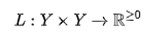
\includegraphics[width=6cm]{./images/1}\par\vspace{1cm}

donde Y es el codominio de g, y L es una función mapas en el número no negativo real s (nuevas restricciones pueden ser colocados enL) . La cantidad L(z,y) es la pérdida sufrida en la predicción de z , como el valor de g cuando su valor verdadero es y.

El riesgo asociado con una función f es la esperanza de la función de pérdida:

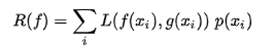
\includegraphics[width=8cm]{./images/2}\par\vspace{1cm}

Si la distribución de probabilidad p es discreta se puede reescribir la fórmula anterior usando una integral en lugar de un sumatorio.
Ahora el objetivo es encontrar una función f* entre una subclase fijo de funciones para las que el riesgoR( f *) es mínima .
Sin embargo, dado el comportamiento de los g generalmente solo es conocido por un conjunto finito de puntos (x1, y1), ..., (xnyn), uno sólo puede aproximar el verdadero riesgo, por ejemplo, con el riesgo empírico:

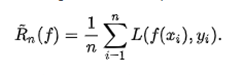
\includegraphics[width=8cm]{./images/3}\par\vspace{1cm}

Selección de la función f* que minimiza el riesgo empírico se conoce como el principio de minimización empírica de riesgos. Teoría estadística de aprendizaje investiga bajo qué condiciones la minimización del riesgo empírico es admisible y lo bien que la aproximación se puede esperar que sea.

\subsection{Aprendizaje Activo}
Hay situaciones en las que el dato sin etiqueta es abundante, pero el dato de etiquetado es caro. En esta situación, el algoritmo de aprendizaje de manera activa la consulta del usuario / profesor para las etiquetas. Este tipo de aprendizaje supervisado iterativo se llama aprendizaje activo. Dado que el estudiante elige los ejemplos, el número de ejemplos para aprender un concepto a menudo pueden ser mucho menores que el número requerido en el aprendizaje supervisado normal. Con este enfoque se corre el riesgo de que el algoritmo puede centrarse en importancia ni como ejemplos válidos.
El aprendizaje activo puede ser especialmente útil en problemas de investigación biológica, como ingeniería de proteínas, donde unas pocas proteínas han sido descubiertos con una cierta función interesante y se quiere determinar cuál de las muchas posibles mutantes que el próximo que tendrá un. 

\subsection{Definiciones}
Que es el conjunto total de todos los datos en cuestión. Por ejemplo, en un problema de ingeniería de proteínas,  se incluyen todas las proteínas que se sabe que tienen una determinada actividad interesante y todas las proteínas adicionales que uno podría querer poner a prueba para esa actividad.

\begin{itemize}
\item Puntos cuya etiqueta es conocida
\item Puntos cuya etiqueta es desconocida
\item Un subconjunto de  escogido para ser etiquetado
\end{itemize}

La mayoría de las investigaciones actuales en el aprendizaje activo implica que el mejor método para elegir los puntos de datos para .

\subsection{Hiperplano marginal mínima}
Algunos de los algoritmos de aprendizaje activo se basan en máquinas de vector soporte y aprovechar la estructura de la SVM para determinar qué puntos de datos a la etiqueta. Estos métodos suelen calcular el margen, de cada dato sin etiqueta en  y tratar  como una distancia n-dimensional a partir de ese dato a la separación de hiperplano.
métodos mínima marginal Hiperplano suponer que los datos con> los más pequeños  son las que el SVM es más seguro acerca de, por lo que debe ser colocado en  se etiqueten. Otros métodos similares, como máximo marginal Hiperplano, elija los datos con> el mayor . métodos de relaciones de intercambio elegir una combinación de la menor y la mayor  s.

\subsection{Máxima curiosidad}
Otro método de aprendizaje activo, que normalmente se entera de un conjunto de datos con menos ejemplos de mínima Hiperplano marginal, pero es más intensivo en cómputo y sólo para los clasificadores discreto es máxima curiosidad.
curiosidad máxima tiene en cada uno sin etiqueta de referencia en  y asume todas las etiquetas posibles ese dato pueda tener. Este dato supone con cada clase se añade a  y luego el nuevo  cruz validados. Se supone que cuando el dato es emparejado con su etiqueta correcta, la exactitud de validación cruzada (o correlación coeficiente) de  mejorará más. El dato con la precisión que más ha mejorado se coloca en  se etiqueten.

\subsection{Aprendizaje Supervisado: Funcionamiento y Tipos}
La primera modalidad de aprendizaje que tiene el machine learning es la de aprendizaje supervisado. Usándola, se entrena al algoritmo otorgándole las preguntas, denominadas características, y las respuestas, denominadas etiquetas. Esto se hace con la finalidad de que el algoritmo las combine y pueda hacer predicciones.
Existen, a su vez, dos tipos de aprendizaje supervisado:
Regresión: tiene como resultado un número específico. Si las etiquetas suelen ser un valor numérico, mediante las variables de las características, se pueden obtener dígitos como dato resultante.


\begin{itemize}
\item Regresión: tiene como resultado un número específico. Si las etiquetas suelen ser un valor numérico, mediante las variables de las características, se pueden obtener dígitos como dato resultante.

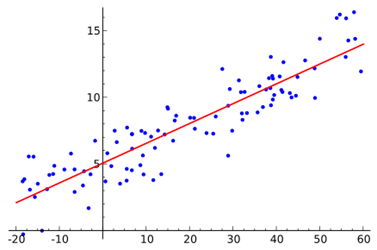
\includegraphics[width=12cm]{./images/4}\par\vspace{1cm}

\item Clasificación: en este tipo, el algoritmo encuentra diferentes patrones y tiene por objetivo clasificar los elementos en diferentes grupos.

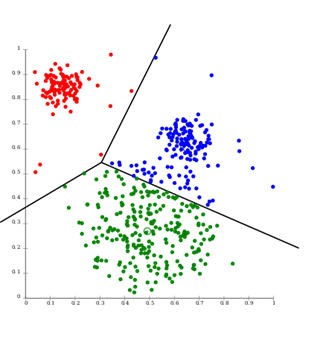
\includegraphics[width=12cm]{./images/5}\par\vspace{1cm}

El algoritmo no está en capacidad de determinar a qué grupo pertenece un valor o cuál es el resultado de una operación. Solamente logra relacionar características con etiquetas y así obtener un resultado.
\end{itemize}


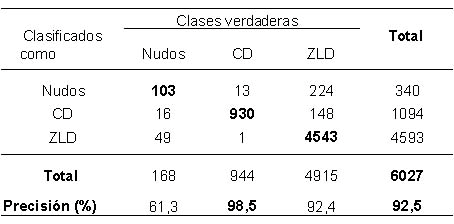
\includegraphics[width=7cm]{./images/6}\par\vspace{1cm}

Uno de los beneficios de las matrices de confusión es que facilitan ver si el sistema está confundiendo dos clases, no solo el error global que comete de saber cuántos ha clasificado bien o no. 
Cuando la máquina se usa para hacer predicciones numéricas (o vectoriales), no clasificación, suele ser normal medir la media del error cometido en los ejemplos de DvalDval, y hablamos del error de validación:

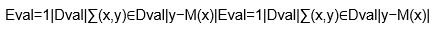
\includegraphics[width=7cm]{./images/7}\par\vspace{1cm}

donde yy sería el valor que se debería haber devuelto, y M(x)M(x) es el valor que nuestra máquina entrenada ha conseguido devolver. Obsérvese que esta fórmula vale para cualquier tipo de resultado en el que podamos medir lo que se diferencia el valor obtenido del esperado. En el caso de los clasificadores sería equivalente a considerar que vale 11 si son distintos, y 00 si son iguales.
Podríamos haber calculado de igual forma el error de entrenamiento, EtrainEtrain, que habitualmente será muy reducido ya que el algoritmo de aprendizaje modifica los parámetros del modelo para intentar minimizarlo. Cuando el proceso consigue reducir este error tanto que es posible que no generalice bien (es decir, al modelo se ha ajustado tanto a los datos vistos, que ha perdido el patrón general que pueden seguir), se dice que se ha producido un sobre-entrenamiento (overfitting), y el modelo resultante deja de ser útil para el propósito inicial de predecir el comportamiento en las partes no observadas.

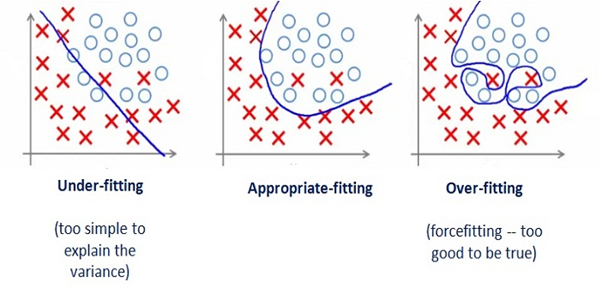
\includegraphics[width=14cm]{./images/8}\par\vspace{1cm}

Por ello, es importante mantener un equilibrio en el proceso de aprendizaje para que no aprenda tanto de los datos proporcionados como para distorsionar el posible patrón general que está detrás de ellos (y que muchas veces tienen un ruido o un sesgo que no podemos evitar en la medición).

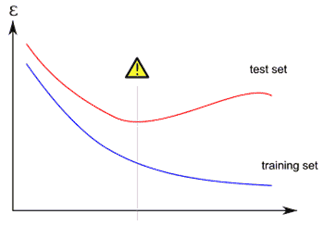
\includegraphics[width=10cm]{./images/9}\par\vspace{1cm}

Ejemplo:
\subsubsection{Medir la eficiencia de un aprendizaje}
Una vez que tenemos una máquina de aprendizaje que es capaz de desempeñar su tarea hemos de pasar a medir la eficiencia de la máquina, es decir, intentar extraer alguna medida que nos informe de lo bien (o mal) que lo está haciendo. Como en los casos de aprendizaje supervisado y no supervisado los objetivos que se buscan son muy distintos, las eficiencias de unos u otros algoritmos suelen definirse también de formas muy distintas.
El caso del aprendizaje supervisado es el más natural y habitual para calcular la eficiencia de la máquina resultante. Recordemos que, en este caso, disponemos de un conjunto de ejemplos iniciales sobre los que realizamos el aprendizaje. Como los algoritmos de aprendizaje supervisado aprenden de estos datos para ajustar sus parámetros internos y devolver la respuesta correcta, no tiene mucho sentido medir la eficiencia de la máquina volviendo a pasarle los mismos datos, ya que la información que nos daría sería engañosamente optimista. Lo que buscamos es ver si la máquina es capaz, a partir de los ejemplos entrenados, generalizar el comportamiento aprendido para que sea suficientemente buena sobre datos no vistos a priori. Si es así, decimos que la máquina (modelo, algoritmo) generaliza correctamente. 

La forma más común para medir esta capacidad de generalización es guardando algunos de los ejemplos iniciales para ser usados posteriormente como validación de la máquina aprendida. Es decir, el conjunto de ejemplos (de los que conocemos el resultado que debe dar), DD, se particiona en dos subconjuntos, de forma que al algoritmo de entrenamiento solo se le enseñan los ejemplos de DtrainDtrain, y una vez realizado el entrenamiento completo, se mide cómo de buenos son los resultados sobre los datos de DvalDval, que nunca ha visto. El error cometido se mide teniendo en cuenta el resultado que la máquina devuelve sobre ellos y el dato, conocido, que debería haber devuelto.
Así, si la máquina es de clasificación, es habitual hablar de la matriz de confusión que se obtiene, que simplemente indica, para cada una de las posibles clases, cuántos ejemplos de DvalDval se clasifican en cada una de las posibles opciones: cada columna de la matriz representa el número de predicciones de cada clase, mientras que cada fila representa las instancias en la clase real. 


\newpage
\section{Análisis}

Las técnicas que utilizan el espectro disperso tienen varias desventajas identificables, una de ellas es un punto flaco en su función de costo. Estos métodos también se ven afectados por la maldición de la dimensionalidad, el número de datos que es requerido para caracterizar la variedad apropiadamente crece a medida que crece la dimensionalidad intrínseca de la variedad. Esta susceptibilidad a la dimensionalidad es una debilidad fundamental en los métodos de aprendizaje local. Otra de las susceptibilidades de este tipo de métodos según (Van Der Maaten, Postma y Van Den Herik 2009) es la predisposición al sobre entrenamiento (lo cual ha sido solucionado parcialmente con métodos adaptativos de vecindad o e-neighboors); la condición de linealidad local asume que las variedades no contienen discontinuidades y la sensibilidad al trabajar con variedades que no son isométricas a un espacio Euclidiano.
De los métodos de enfoque disperso, uno de los más populares lo constituye LLE, el cuál ha sido ampliamente aplicado en varias áreas (Ziegelmeier, Kirby y Peterson 2012; Yang, Xiang y Shi 2013; Liu et al. 2013). En los últimos años algunos autores han profundizado en la selección del parámetro de vecinos más cercanos obteniendo buenos resultados (Castellanos Domínguez et al. 2011; Karbauskait, Kurasova y Dzemyda 2015). Sin embargo, LLE es débil ante las irregularidades de la variedad al ser un método local, y debido a la simplicidad de la restricción de covarianza en su solución es propenso a redimensiones en la variedad en el proceso de embebido.
Si bien la distancia geodésica podría resultar útil para añadir expresividad a los datos y explorar mayor información en conjuntos de datos complejos; ISOMAP tiene desventajas, entre ellas, la inestabilidad topológica (Balasubramanian 2010) que provoca que construya conexiones erróneas en el grafo de vecindad, lo que podría afectar su desempeño, la presencia de espacios "vacíos" en la variedad, o la susceptibilidad a variedades no convexas. Sin embargo, varios autores han utilizado este método o variaciones del mismo debido a la expresividad que facilita la información topológica que proveen las distancias geodésicas (Hu, Lu y Xu 2012; Hauberg, Freifeld y Black 2012; Wang, Yuen y Feng 2012).
El método de aprendizaje adaptativo no lineal de métricas de distancia (Non-linear adaptative metric learning; NAML) (Chen et al. 2007) realiza agrupamiento y aprendizaje de distancias simultáneamente.
Primero mapea los datos a un espacio de mayor dimensión a través de una función núcleo, y luego aplica una proyección lineal para encontrar una variedad de menor dimensión donde se maximice la separabilidad de los datos, en ese espacio es donde se realiza el agrupamiento. Este algoritmo ha tenido buenos resultados en comparación con otros métodos del estado del arte como LLE y LE. Los métodos de aprendizaje no supervisado de distancias en un espacio de núcleo compuesto (Unsupervised distance metric learning in composite kernel space; CKS-EWFC-K, CKS-EWFC-F) (Wang et al. 2016) se combinan en una plataforma de desarrollo de agrupamiento difuso y aprendizaje de métricas de distancia. Los algoritmos obtienen la función de distancia usada para el cálculo de la similitud a través de un proceso de aprendizaje no supervisado durante el proceso de agrupamiento del sub-espacio suavizado. Tanto NAML como los recientes CKS-EWFC-K y CKS-EWFC-F pueden adaptarse a los datos para aprender funciones de distancia acordes a los conjuntos de datos durante el proceso de agrupamiento. Sin embargo, aún se encuentran en fase de estudio experimental para el ajuste de los parámetros y las guías de identificación de los mismos.


\newpage
\section{Conclusiones}
El desarrollo de métodos para el aprendizaje de funciones de distancia a partir de los datos ha tenido un desarrollo imponente en los últimos años. En su mayoría los enfoques se caracterizan por formular un problema de optimización a partir de restricciones que se obtienen de las instancias de aprendizaje. El proceso de minimización o maximización de la función objetivo que codifica las restricciones se realiza mediante un costoso algoritmo iterativo. Estos métodos, cuando se utilizan de conjunto con un clasificador vago como el k-NN, permiten incrementar la calidad de la clasificación al costo de una complejidad computacional alta. En el estudio realizado se abordaron aspectos generales del aprendizaje de funciones de distancia, así como su aplicabilidad a la mejora de algoritmos de clasificación basados en instancias. Dentro del enfoque supervisado se distinguieron dos categorías que dependen de la forma en que se obtienen las restricciones, esto es, en la vecindad de cada instancia (local) o en todo el espacio de representación (global). En cada categoría se detallaron las ideas detrás de las implementaciones de los algoritmos más representativos. Este trabajo resulta de utilidad para comprender la esencia del aprendizaje de funciones de distancia y facilita la selección de que algoritmos aplicar dada la disponibilidad de información en forma de restricciones.

\section{Webgrafia}

\begin{itemize}
\item http://www.cs.us.es/~fsancho/?e=77
\item https://medium.com/@juanzambrano/aprendizaje-supervisado-o-no-supervisado-39ccf1fd6e7b
\end{itemize}

\end{document}